\subsection{Examples of Siumatgwoons}

What are some examples of Siumatgwoons? 




\subsubsection{The Chinese Characters, 字}

The Chinese characters, which inspired this whole mathematical exercise, is clearly a Siumatgwoon. If we exercise the synonym exchange of "Siumatgwoon" with "Metaphysic", this is to say, that the Chinese characters is a Metaphysic. Unfortunately we can't really \textit{prove} that the Chinese characters are indeed a siumatgwoon, given there's an infinite number of them, and we do not have a generating rule for all Chinese characters. However, the fact that any subset of Chinese characters is a siumatgwoon in of itself, lends us confidence - perhaps there's a theorem there waiting to be proved?


\subsubsection{The Roman Numerals $\mathfrak{R}$}

One can clearly see that Roman Numerals $\mathfrak{R}$ are a Siumatgwoon. However, to appreciate the characteristics that make it a Siumatgwoon, let us consider the subset of Roman Numerals from 1 to 10, which we shall show to also be a Siumatgwoon.

$\mathfrak{R}_{1,10} = \{I, II, III, IV, V, VI, VII, VIII, IX, X\}$

We will say that for two elements $a,b \in \mathfrak{R}_{1,10}$, $a|b$ iff the glyph $a$ appears in $b$. As such, we can say $I | II$ and $I|III$ as an example, and that $V|IV$ and $X|IX$. 

For any elements $a,b\in \mathfrak{R}_{1,10}$, if the glyphs $ab$ so written together forms a glyph that also appears in $\mathfrak{R}_{1,10}$, then we'd say that $a*b\in \mathfrak{R}$.

Now, it's clear that Ax 1 is satisfied trivially. 

Ax 2 is also satisfied trivially.

Ax 3 is also satisfied. 

Ax 4 is also satisfied. As an example: $I | III, III | VIII$ and we have $I|VIII$.

So therefore, $\mathfrak{R}_{1,10}$ is a Siumatgwoon. 

It is also interesting to note that as per the definition of $\mathfrak{R}_{1,10}$, it is not compositionally closed. For example, $II * III$ is not in $\mathfrak{R}_{1,10}$. This makes the Siumatgwoon different from a group, where all compositions are contained inside the group. Intuitively, perhaps this suggests the Siumatgwoon is less rich in structure than the mathematical group? Also, note that what $II * III$ should be in $\mathfrak{R}_{1,10}$ is represented by $V$. Intuitively, we can feel that in some sense, $II * III = V$ - that they're synonymous, identical, referring to the same referent. This is not unlike the presence of variant characters in the Sinoglyphs, such as 體 (body, object)=骵=躰=体, or信 (trust) = 𬢭 = 伩 = 訫 = 㐰… Intuition should hint that this will yield some interesting structures if we pursue the investigation down this path.

\subsubsection{Any Numerals System}

The fact that the Roman Numerals are a Siumatgwoon should intuitively suggest that any numeral system is a Siumatgwoon. In fact, let us consider the world's many numeral systems, and see if there is one where it is not a siumatgwoon. 

\begin{center}
\begin{tabular}{|l|c|c|c|c|c|c|c|c|c|c|}
\hline
 & 0 & 1 & 2 & 3 & 4 & 5 & 6 & 7 & 8 & 9 \\
\hline
唐字數字 & 〇 & 一 & 二 & 三 & 四 & 五 & 六 & 七 & 八 & 九 \\
\hline
唐字數字大寫 & 零 & 壹、弌 & 貳 & 叄 & 肆 & 伍 & 陸 & 柒 & 捌 & 玖 \\
\hline
字喃 &  & 𠬠 & 𠄩 & 𠀧 & 𦊚 & 𠄼 & 𦒹 & 𦉱 & 𠔭 & 𠃩 \\
\hline
蘇州碼子 & 〇 & 〡、一 & 〢、二 & 〣、三 & 〤 & 〥 & 〦 & 〧 & 〨 & 〩 \\
\hline
Roman Numerals &  & I & II & III & IV & V & VI & VII & VIII & IX \\
\hline
Eastern Arabic & ٠ & ١ & ٢ & ٣ & ٤ & ٥ & ٦ & ٧ & ٨ & ٩ \\
\hline
Persian & ٠ & ۰ & ۱ & ۲ & ۳ & ۴ & ۵ & ۶ & ۷ & ۸ \\
\hline
Devanagari & ० & १ & २ & ३ & ४ & ५ & ६ & ७ & ८ & ९ \\
\hline
Gujarati & ૦ & ૧ & ૨ & ૩ & ૪ & ૫ & ૬ & ૭ & ૮ & ૯ \\
\hline
Tibetan & ༠ & ༡ & ༢ & ༣ & ༤ & ༥ & ༦ & ༧ & ༨ & ༩ \\
\hline
Hebrew &  & א & ב & ג & ד & ה & ו & ז & ח & ט \\
\hline
Chinese counting rods &  & 𝍠 & 𝍡 & 𝍢 & 𝍣 & 𝍤 & 𝍥 & 𝍦 & 𝍧 & 𝍨 \\
\hline
counting 正 &  & 𝍲 & 𝍳 & 𝍴 & 𝍵 & 𝍶 & 𝍶𝍲 & 𝍶𝍳 & 𝍶𝍴 & 𝍶𝍵 \\
\hline
Tangut &  & 𘈩 & 𗍫 & 𘕕 & 𗥃 & 𗏁 & 𗤁 & 𗒹 & 𘉋 & 𗢭 \\
\hline
\end{tabular}
\end{center}

I don't think there's a single one that's not a siumatgwoon! Most of them are pathological for sure, in the sense that nothing is constituted by anything else, but none of them violate the Siumatgwoon axioms! 

The case of the numerals as a Siumatgwoon, or a Metaphysic, is interesting. Numerals all refer to the same referents, the same "things" or "objects", namely, numbers. However, the glyphs in a given numeral system are themselves imbued with a particular set of metaphysical prejudices and judgements. Under the Roman Numeral Metaphysic, the number 3 is composed of 1 and 2, or composed of three 1s. 4 is composed of 1 and 5, but not 3 and 2. 

\subsubsection{The Polygons $\mathcal{P}$}

Consider the following graph. If we take all the polygons, convex and star, as elements in a set called $\mathcal{P}$, we can see that it forms a Siumatgwoon. We state this without formal proof for the infinite set $\mathcal{P}$, but from the subset displayed in the graph below, we can see it is indeed true. A polygon $a$ constitutes polygon $b$ if $a$ appears in $b$. $\{3\}$, the equilateral triangle, appears in $\{6/2\}$, the star of David, and so $\{3\} |\{6/2\}$



% include images of polygons_1.png and polygons_2.png
\begin{figure}[!htbp]
    \centering
    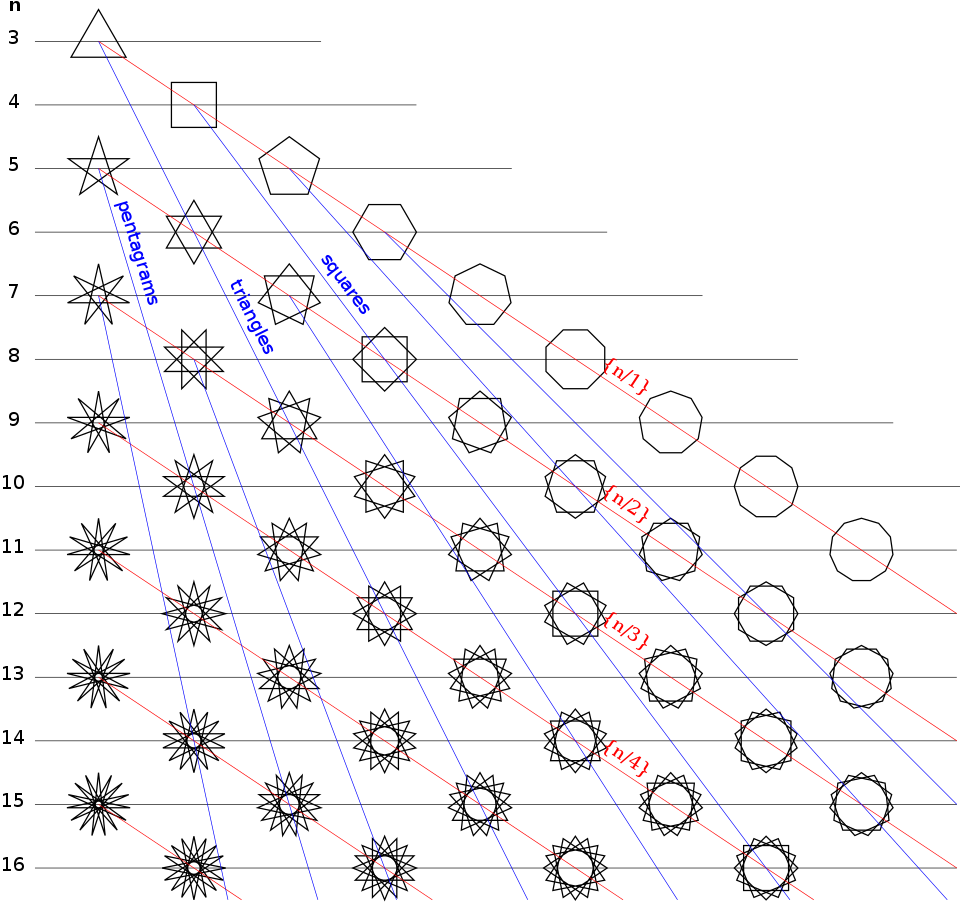
\includegraphics[width=0.8\textwidth]{images/polygons_1.png}
    \caption{A graph of the polygons}
\end{figure}
\begin{figure}[!htbp]
    \centering
    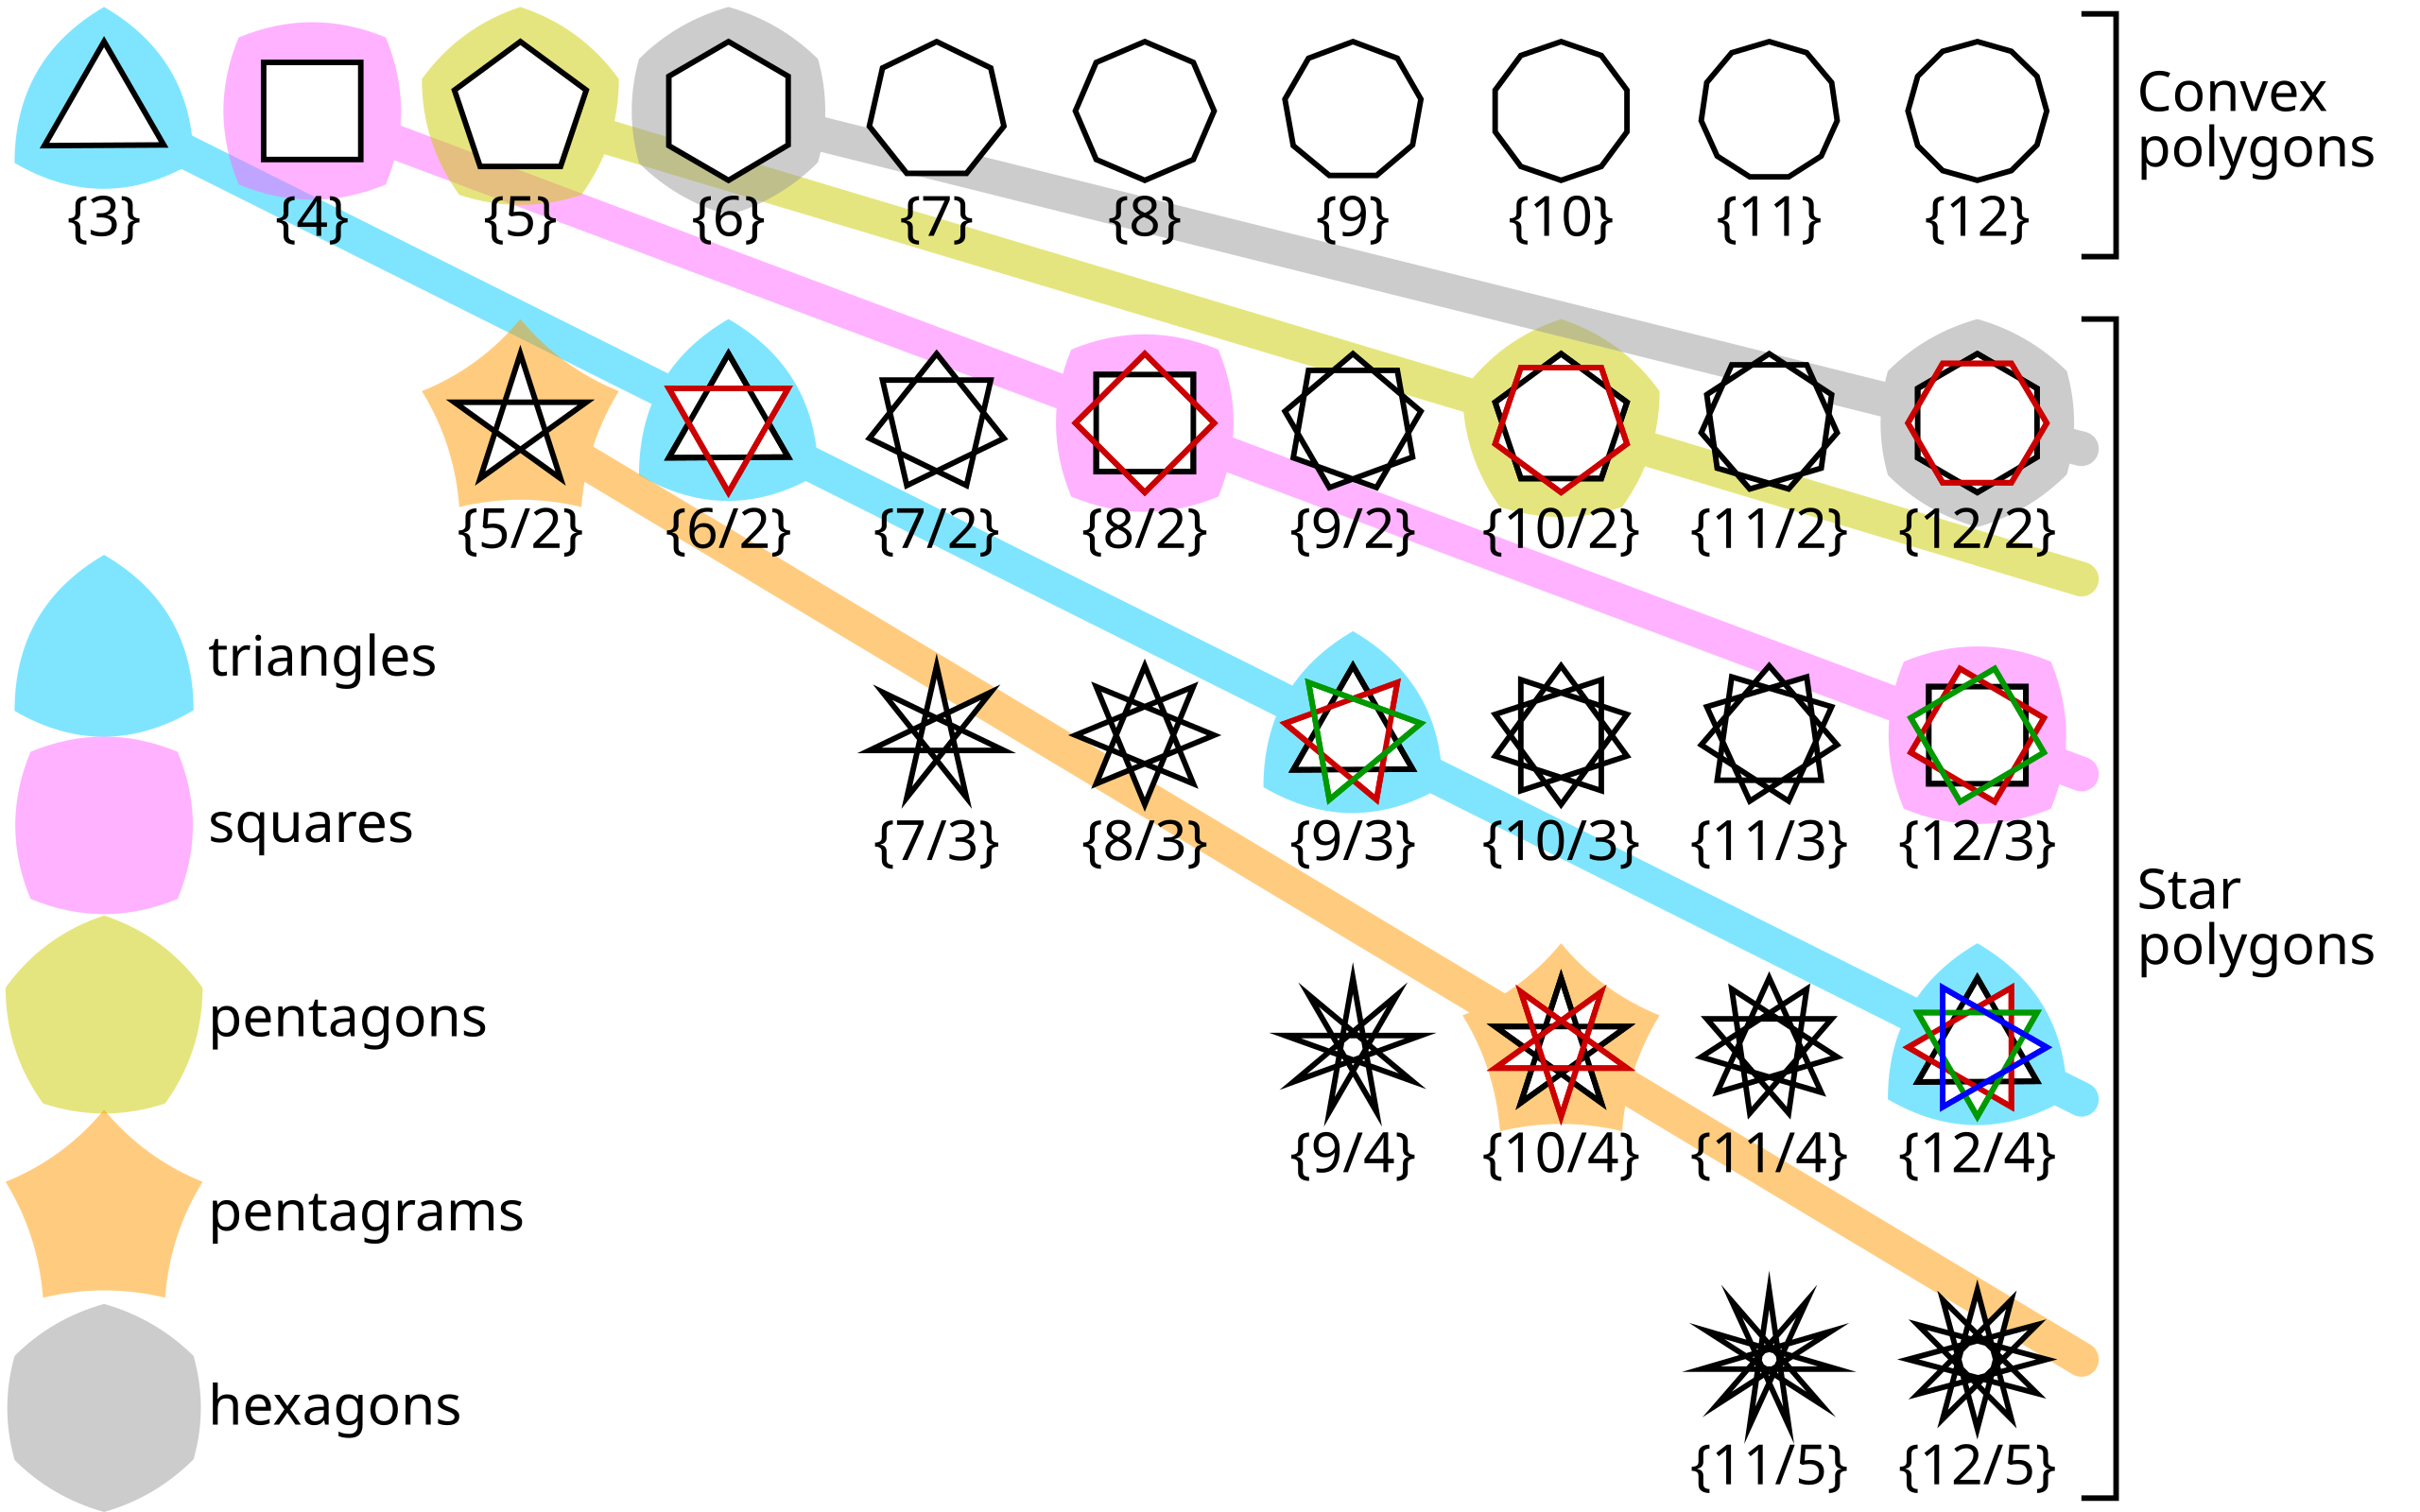
\includegraphics[width=0.8\textwidth]{images/polygons_2.png}
    \caption{A graph of the polygons}
\end{figure}


The Schläfli symbol is a recursive description, starting with $\{p\}$ for a $p$-sided regular polygon that is convex. For example, $\{3\}$ is an equilateral triangle, $\{4\}$ is a square, $\{5\}$ a convex regular pentagon, etc.

Regular star polygons are not convex, and their Schläfli symbols take the form $\{p/q\}$, where $p$ is the number of vertices and $q$ is their turning number. Equivalently, $\{p/q\}$ is created from the vertices of $\{p\}$ by connecting every $q$th vertex. For example, $\{5/2\}$ is a pentagram, while $\{5\}$ is a pentagon.

Note that $p$ and $q$ must be coprime, or the figure will degenerate, in which case we have the following theorem:

$\{p/q\}=d\{ \frac{p}{d} / \frac{q}{d} \}$, where $d=\gcd(p,q)$.

Let us define for any Schläfli symbol $\{p\} | n\{p\}$ for any $n$. It is intuitively true.

Then clearly axiom 1 is satisfied. Axiom 2 is also satisfied.

\subsubsection{Propositional Logic}

There are 3 flavors of $*$ in Propositional Logic: $\wedge, \vee, \rightarrow$. 

And we define $\phi | \psi$ if $\phi$ appears in $\psi$, for any wff $\phi, \psi$.

Then clearly all 4 of the core siumatgwoon axioms are satisfied. 

\begin{enumerate}
\item Trivial that all $\phi | \phi$
\item Also trivial that for any $\phi, \psi$, either $\phi|\psi$ or $\phi\not|\psi$.
\item Trivial as well that for any $\phi,\psi | \phi * \psi$.
\item Also trivial that if $\phi | \psi$ and $\psi | \theta$ then $\phi | \theta$.
\end{enumerate}

Propositional Logic as a Siumatgwoon has multiple interesting properties: 

\begin{enumerate}
\item It is compositionally complete. 
\item It is also constitutionally complete. 
\item Is it a simple siumatgwoon? Are decompositions finite? Yes. Are decompositions unique? Yes, up to reordering. So yes, it's a simple siumatgwoon.


\end{enumerate}

